%\section{Bifurcations, Tipping points and catastrophes.}





%Tipping points are situations where a system suddenly flips between two stable states, one becoming unstable (end of branch in phase diagram) \ref{fig: supercritical pithfork}. 




%Abrupt transitions can also occur in systems where the output depends linearly, but with a high (or even infinite) slope\cite{..}.


\section{Critical slowing down and resilience}


To provide an EWS to such transitions, dynamical or model-based approaches have been proposed, in particular related to the effect of critical slowing down \citep{Scheffer2009,Scheffer344,doi:10.1111/j.1600-0706.2012.20838.x}, where the time to recover the stable state of a system after a perturbation increases near a transition.



%However these dynamical approaches impose to observe the system evolution over time after a perturbation. 
%Coupled to the emergency to take decision, this may make forecast unpractical and can be very sensitive to noise. 
%Also, this is very sensitive to noise. 


In general, a dynamical system is described by a system of first order differential equations (ODE's):

\begin{equation}
\dot{\vec x}=\vec f(\vec x,\vec\la,t)
\label{eq: ODES}
\end{equation}

where $\vec x=(x_1,\dots,x_n)$ and $\vec f=(f_1(\vec x,\vec \la ,t),\dots,f_n(\vec x,\vec \la ,t))$ is at least a $C^1$  functions\footnote{\textcolor{red}{Because i don't know how much of this holds for frictional systems. }We are not working with non-smooth ODES or discrete maps.}, $\vec\la$ a set of control parameters and $t$ is the evolution variable (time in this case).


\begin{figure}[htb]
	\begin{center}
		\begin{tikzpicture}[scale=1.5, every node/.style={scale=1.5}]
			\tzaxes(-1.5,-1.4)(1.5,1.4){$x$}{$\dot{x}$}
			\tzfn[col2,thick]{(0.5*\x+\x^3-\x^5)}[-1.25:1.25]{$\la=0.5$ }[ar]
			\tzfn[col2,thick]{(-0.5*\x+\x^3-\x^5)}[-1.25:1.25]{$\la=-0.5$ }[ar]
			\tzfn[col2,thick]{(-0.1*\x+\x^3-\x^5)}[-1.25:1.25]{$\la=-0.1$ }[ar]
			%	\draw [->,thick](0.8,0) -- (0.3,0);
			%	\draw [->,thick](-0.8,0) -- (-0.3,0);
			%	\draw [->,thick](1.2,0) -- (1.5,0);
			%	\draw [->,thick](-1.2,0) -- (-1.5,0);
			%	\node (a) at (0,0) {};
			%	\filldraw (a.center) circle [radius=0.1cm];
			%	\draw (a)+(1,0) circle [radius=0.1cm];
			%	\draw (a)+(-1,0) circle [radius=0.1cm];
		\end{tikzpicture}  \qquad \qquad
		\begin{tikzpicture}[scale=1.5, every node/.style={scale=1.5}]
			%	\tzaxes(-0.5,-2)(2,2){$x$}{$r$}
			\tzfn[black,very thick]{sqrt(0.5)*sqrt(1+sqrt(1+4*\x))}[-0.249:0.7]{}[ar]	
			\tzfn[black, very thick]{-sqrt(0.5)*sqrt(1+sqrt(1+4*\x))}[-0.249:0.7]{}[ar]
			\tzfn[black,dashed,thick]{sqrt(0.5)*sqrt(1-sqrt(1+4*\x))}[-0.249:0]{}[ar]	
			\tzfn[black,dashed,thick]{-sqrt(0.5)*sqrt(1-sqrt(1+4*\x))}[-0.249:0]{}[ar]
			\draw [-,very thick](-0.8,0) -- (0,0);
			\draw [dashed,thick](0,0) -- (0.7,0);
			\draw [->,semithick,opacity=0.4](-0.5,0) -- (1.4,0)  node[right] {$\la$};
			\draw [->,semithick,opacity=0.4](0,-1.4) -- (0,1.4) node[above] {$x^*$} ;
			\draw [col1,->,very  thick](0.026, 0.22) -- (0.026, 0.71 + 0.1);
			\draw [col1,->,very  thick](-0.29, 0.71) -- (-0.29,0.1);
			%			\node (a) at (0,0) {};
			%	\node[circle,draw,minimum size=10cm] (a) at (0,0) {};
			%			\draw (a.center) circle [radius=0.1cm];
			%			\filldraw (a)+(1,0) circle [radius=0.1cm];
			%			\filldraw (a)+(-1,0) circle [radius=0.1cm];
			%	\tzfn'[red,thick]{(\x)^2}[-1:2]{$f^{-1}(x)$}\\[ar] % inverse
		\end{tikzpicture}
	\end{center}
	\caption{Stability of $\dot{x}=\la x+x^3-x^5$. Between $\la=-0.25$ and $\la=0$ the system has three stable branches, while, after $\la=0$ the branch at $x=0$ becomes unstable. This means that in the region  $\la=(-0.25,0)$ the system presents hysteresis. \textcolor{red}{maybe i shuold choose if i keep this or fig 4.2, not both} }
	\label{fig: supercritical pithfork}
\end{figure}


If eq.\eqref{eq: ODES} has a set of equilibria or fixed points \footnote{ $\vec{x}(t)=\vec{x}^*$ such that $\dot{\vec{x}}=0$.  }, $ \left\lbrace \vec{x}^*_1,\dots, \vec{x}^*_k \right\rbrace $, then a Taylor expansion around this points gives 

\begin{equation}
\dot{\vec x}(x\approx x^*,t)\approx \vec f(\vec{x}^*,t)+ \vec{\nabla}  \vec f(\vec{x}^*,t)(\vec{x}-\vec{x}^*)+ \frac{1}{2} \vec{\nabla} \vec{\nabla} \vec f(\vec{x}^*,t)(\vec{x}-\vec{x}^*)^2+\dots 
\label{eq: EWS_taylor}
\end{equation}
where $\vec{x}^*=(x^*_1,\dots,x^*_n)$ is an equilibrium; and  
\begin{equation}
	\vec{\nabla}  \vec f(\vec x^*,t)=M=
	\begin{bmatrix}
		\frac{d f_1}{d x_1}\hdots \frac{d f_1}{d x_n}  \\
		\vdots \\
		\frac{d f_n}{d x_1}\hdots \frac{d f_n}{d x_n}
	\end{bmatrix}
\end{equation}
is the Jacobian of $\vec f$, also called   the linear decay rate (LDR) when $\vec{x}^*(\la)$ is a stable state of the system.
Here we will call $m_j$ the eigenvalues of $M$, and we will call $||M||$  the maximum eigenvalue $m_{max}=\max \left\lbrace m_j \right\rbrace $.
If the system is near a stable equilibrium, and we assume there is a clear separation of scales, that is $||M||$ much larger than the other eigenvalues, then the system is dominated by the slowest timescale (the relaxation time) defined as   
\begin{equation}
	t^*=-\frac{1}{||M(x^*)||}.
\end{equation}

Under this assumptions the system behaves locally as a 1-dimensional system. Therefore we drop the vector notation from now on, unless needed, and we use $M$ and $||M||$ as the same \textcolor{red}{this is not the phrasing you are looking for} .

Since we are close to the stable equilibrium $x^*$, at first order we get 
\begin{equation}
	f|_{x^*}=\cancelto{0}{f(x^*)}+f'(x^*)(x-x^*) \rightarrow \dot{x}|_{x^*}=M(x^*)(x-x^*)
\end{equation}
where the prime denotes differentiation with respect to $x$.

This gives us a local behavior  
\begin{equation}
	x(x\approx x^*)=A e^{M(x^*)t}+x^*
\end{equation}
where $A$ is an integration constant depending on the initial condition. 

We call a co-dimension-1 critical transition, a bifurcation where, as the system approaches a bifurcation point defined by a single control parameter value $\la=\la_c$, the return rate approaches $0$.

\begin{figure}[htb]
	\begin{center}
		\begin{tikzpicture}[scale=2, every node/.style={scale=1.6}]
			%	\tzaxes(-0.5,-2)(2,2){$x$}{$r$}
			\tzfn[black,ultra thick]{sqrt(0.5)*sqrt(1+sqrt(1+4*\x))}[-0.249:0.9]{}[ar]	
			%		\tzfn[black,ultra thick]{-sqrt(0.5)*sqrt(1+sqrt(1+4*\x))}[-0.249:0.9]{}[ar]
			\tzfn[black,dashed, ultra thick]{sqrt(0.5)*sqrt(1-sqrt(1+4*\x))}[-0.249:0]{}[ar]	
			%	\tzfn[black,dashed,very thick]{-sqrt(0.5)*sqrt(1-sqrt(1+4*\x))}[-0.249:0]{}[ar]
			\draw [-,ultra thick](-1.7,0) -- (0,0);
			\draw [dashed, ultra thick](0,0) -- (0.9,0);
			\draw [->,thin,opacity=0.4](-0.5,0) -- (1.4,0)  node[right] {$r$};
			\draw [->,thin,opacity=0.4](0,-0.1) -- (0,1.7) node[above] {$x^*$} ;
			
			%		\coordinate (c1) at ((0.5^(0.5))*(1+(1+4*0.9)^(0.5))^(0.5));
			
			\draw [->,ultra thick,col1](-1, 0.7) -- (-1, 0.1);
			\draw [->,col1,thick, opacity=0.8](-0.4, 0.5) -- (-0.4,  0.1);
			\draw [->,col1,semithick, opacity=0.6](-0.1, 0.3) -- (-0.1,  0.1);
			
			\draw [->,ultra thick,col2](0.8, 1.9) -- (0.8,  1.9-0.6);
			\draw [->,col2,thick, opacity=0.8](0.2, 1.55) -- (0.2,  1.55-0.4);
			\draw [->,col2,semithick, opacity=0.6](-0.15, 1.2) -- (-0.15,  1.2-0.2);
			%			\node (a) at (0,0) {};
			%	\node[circle,draw,minimum size=10cm] (a) at (0,0) {};
			%			\draw (a.center) circle [radius=0.1cm];
			%			\filldraw (a)+(1,0) circle [radius=0.1cm];
			%			\filldraw (a)+(-1,0) circle [radius=0.1cm];
			%	\tzfn'[red,thick]{(\x)^2}[-1:2]{$f^{-1}(x)$}\\[ar] % inverse
		\end{tikzpicture}
	\end{center}
	\caption{Relaxation time changes approaching the bifurcation, pictured by the thickness of the arrows in each stable branch. \textcolor{red}{it would be better with a cool/warm colormap for stable/unstable and real values.} }
	\label{fig: relax time.}
\end{figure}

Critical slowing down (CSD) is the slowing down of relaxation times near a stable solution when the system is near a bifurcation. In other words, it is the loss of resilience of the stable manifold near a transition. 

This is usually pictured as the potential of a system with enough damping to have overdamped solutions, defined as $V=-\int dx\,f(x,\la)$. In this picture, as the system approaches the bifurcation, it looses stability (the potential well becomes more shallow \footnote{It might also become more narrow, in which case the tipping might also happen due to a change in the basin. Though we do not focus on this cases.} ) which means a perturbation might send the system to another stable state, as pictured in figure \ref{fig: resiliance_and_csl}.


\begin{figure}[htbp]
	\begin{center}
		\begin{tikzpicture}
			\tzaxes(0,0)(5,4){State}{Potential}
			\tzfn[black,very thick]{2*(\x-1)^2*(\x-3)^2+0.5*\x}[0.6:3.4]{ }[ar]
			\tzfn[<-,black,dashed]{2*(\x-1)^2*(\x-3)^2+0.5*\x+0.3}[1.6:2.7]{ }[ar]
			\tzfn[<-,very thick,col1,dashed]{2*(\x-0.2-1)^2*(\x-0.1-3)^2+0.5*(\x-0.2)-0.1}[3.1:3.4]{ }[ar]
			%			\draw [->,thick](0.8,0) -- (0.3,0);
			%			\draw [->,thick](-0.8,0) -- (-0.3,0);
			%			\draw [->,thick](1.2,0) -- (1.5,0);
			%			\draw [->,thick](-1.2,0) -- (-1.5,0);
			\node (a) at (0,0) {};
			\filldraw [col2,opacity=0.4] (0.97,0.5+0.14) circle [radius=0.1cm];
			\filldraw [col2](2.97,1.5+0.14) circle [radius=0.1cm];
			\filldraw [col2](3.2, 2.06 + 0.5) circle [radius=0.1cm];
			\draw [<->,thick](0.4,1.5)--(0.4,2.9);
			\draw [<->,thick](2.1,0.2)--(2.9,0.2);
			\node (t) at (2.5,3.9) {High resiliance}[c];		
		\end{tikzpicture} 
		\begin{tikzpicture}
			\tzaxes(0,0)(5,4){State}{Potential}
			\tzfn[ black,very thick]{(\x-1)^2*(\x-3)^2+0.7*\x}[0.6:3.4]{ }[ar]
			\tzfn[<-,very thick,col1,dashed]{(\x-1)^2*(\x-3)^2+0.7*\x+0.3}[1.6:2.7]{ }[ar]
			\tzfn[<-,black,dashed]{(\x-0.2-1)^2*(\x-0.1-3)^2+0.7*(\x-0.2)-0.1}[3.1:3.4]{ }[ar]
			%			\draw [->,thick](0.8,0) -- (0.3,0);
			%			\draw [->,thick](-0.8,0) -- (-0.3,0);
			%			\draw [->,thick](1.2,0) -- (1.5,0);
			%			\draw [->,thick](-1.2,0) -- (-1.5,0);
			\node (a) at (0,0) {};
			\filldraw [col2] (0.92,0.7+0.1) circle [radius=0.1cm];
			\filldraw [col2,opacity=0.4](2.92,3*0.7+0.1) circle [radius=0.1cm];
			\filldraw [col2] (3.22, 2.4 + 0.5) circle [radius=0.1cm];
			\draw [<->,thick](0.4,2.1)--(0.4,2.5);
			\draw [<->,thick](2.4,0.2)--(2.9,0.2);
			\node (t) at (2.5,3.9) {Low resiliance}[c];		
		\end{tikzpicture}
	\end{center}
	\caption{As the system (left panel) moves closer to a tipping point, it losses resilience (right panel), and the system might change state (red circle) due to a perturbation that was not enough to force the system to tip to a new equilibrium when it had more resilience.    }
	\label{fig: resiliance_and_csl}
\end{figure}

At the same time as the LDR goes to $0$ as shown in figure \ref{fig: relax time.}, the relaxation time increases, which leads to a slowing down of the dynamics(critical slowing down). 
This means that, in the presence of noise (perturbations), the CSD is manifested as an increase of variance.  
%\begin{figure}
%	\centering
%\begin{tikzpicture}
%	\tzaxes(-0.4,-0.5)(2,3){$x$}{$\dot{x}$}
%	\tzfn[blue,thick]{2*(\x)*(\x-1)^2+0.3}[-0.3:1.5]{$f(x)$}[ar]
%	\draw [->,thick](-0.3,0) -- (-0.6,0);
%	\draw [->,thick](-0.3,0) -- (0.3,0) ;
%	\node (a) at (0,0) {};
%	%	\node[circle,draw,minimum size=10cm] (a) at (0,0) {};
%	\filldraw (a)+(-0.4,0) circle [radius=0.1cm];
%	%	\tzfn'[red,thick]{(\x)^2}[-1:2]{$f^{-1}(x)$}\\[ar] % inverse
%\end{tikzpicture}
%	\caption{Slowing down from ghosting. .. dunno if i should keep this. }
%\label{fig: ghosting}
%\end{figure}






\subsection{Estimation for linearly stable systems in critical bifurcations}
\textcolor{red}{by this i mean bifurcation where the eigenvalue is real}

In particular, if the system is linearly stable, then near the stable point, the system returns as

\begin{equation}
	x(t)=Ae^{-M t}+x^*
\end{equation}

For this, we have to ask for the determinant of the jacobian matrix to be non zero, 
\begin{equation}
	det(M(x^*,\lambda))\neq0
\end{equation}

with $\lambda\neq \lambda_c$. Then, we can do a Taylor expansion of the Jacobian near (before) the bifurcation. 
If the eigenvalues are real,  at the bifurcation the determinant becomes zero and we get:
\begin{equation}
	M(x^*,\la\approx \lambda_c)\approx \cancelto{0}{M(x^*,\lambda_c)}+\partial_\lambda M(x^*,\lambda_c) (\lambda-\lambda_c)+\frac{1}{2}\partial^2_\lambda M(x^*,\lambda_c) (\lambda-\lambda_c)^2+... 
\end{equation}

Thus, near a bifurcation we expect the return time to be 
\begin{equation}
	t^*=-\frac{1}{M}\approx \frac{\kappa_1}{(\lambda-\lambda_c)}+\frac{\kappa_2}{(\lambda-\lambda_c)^2}+\dots
\end{equation}
where $\kappa_j$ are constants related to the different derivatives $\partial^j_\lambda M(x^*,\lambda_c)$.

Therefore, before the bifurcation, the return rate goes as  $1/(\lambda-\lambda_c)$ and as the system gets closer to the bifurcation the higher order terms dominate the return time which diverges geometrically at the bifurcation\footnote{\textcolor{red}{I could think of an example where this coefficients are all $1$ and it gives an exponential series.}}.

% $1/(\lambda-\lambda_c)^n$ and the return time 

\section{Types of tipping}

If we say a system tips when it changes some aspect of its behavior, dynamical systems can display several kind of tipping\footnote{It should be noted that we do not explore bifurcations of the basins of attraction.}.

We can classify this changes according to the mechanism that forces the system to change. This could be because:
\begin{enumerate}
	\item the system crosses a dynamical bifurcation (B-tipping)
	\item   the noise is large enough for the system to be able to reach  the basin of another regime (N-tipping)
	 \item  a parameter is the system is also evolving in time, and this forces the system to either have a new dynamical equilibrium or to tip towards another regime depending on the rate of change of the parameter (R-tipping)
	 \item to external shocks that forces the system to another basin (S-tipping).
\end{enumerate} 

\begin{figure}[htb]
	\centering
	Tipping points
	\hline
	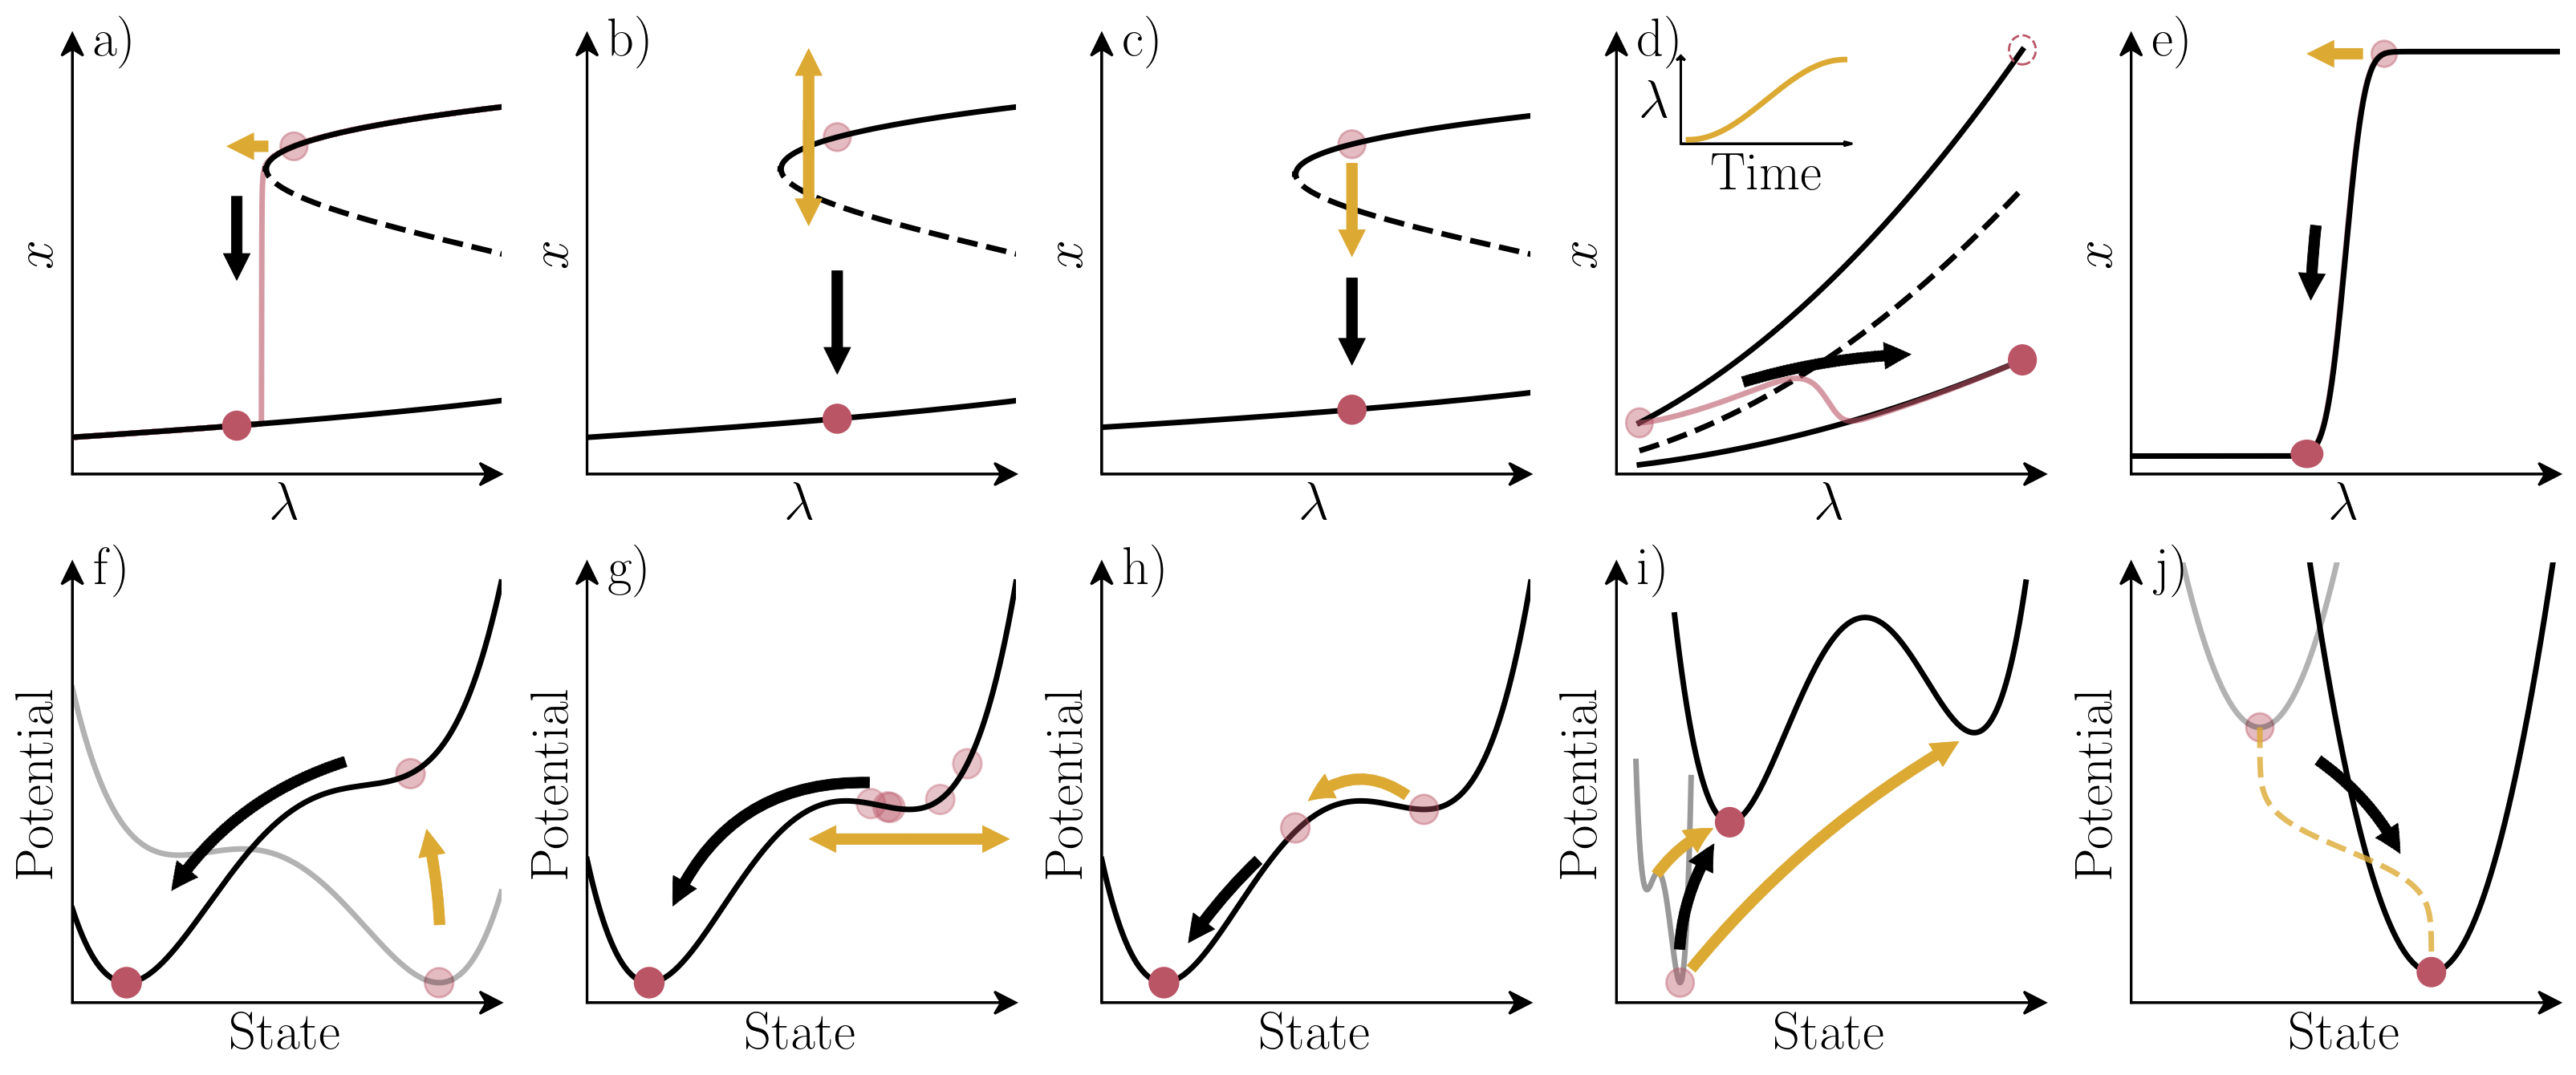
\includegraphics[width=1\linewidth]{Images/Metrics/tippings}
	\caption{Top row shows the effect of the tipping on the bifurcation diagram, while bottom row shows the corresponding potential picture. a, f) Tipping due to bifurcation (B-tipping). b, g) Tipping due to  noise (N-tipping). e, h) Tipping due to a single large perturbation (S-tipping). d, i) Tipping due to a quick change in control parameter (R-tipping). e, j) Tipping due to a fast change in the stable state (quick transition). }
	\label{fig:largetippingsscheffer}
\end{figure}


\subsection{Dynamical bifurcations, or B-tipping}
Following \cite{Thompson2011a}, we can classify codimension-1 bifurcations\footnote{Bifurcations that can be encountered when sweeping or scanning only one control parameter.} on how much the system changes and how hard it is to reverse the system to the previous regime. 
Taking this into account we can  classify them into safe (\cref{tab:safe_bifs}), dangerous (\cref{tab:explos_bifs}), and explosive bifurcations\footnote{Here there might be a few new bifurcations missing...}  (\cref{tab:dangerous_bifs}).


\begin{table}[H]
			\centering
		\begin{tabular}{ll}
			\hline
			\multicolumn{2}{c}{\textbf{Safe bifurcations}} \\
			\textbf{a) Local Supercritical bifurcations} & \\
				1. Supercritical Hopf & Point to cycle\\
				2. Supercritical Neimark-Sacker (secondary Hopf) & Cycle to torus \\				
				3. Supercritical Flip/period doubling & Cycle to cycle \\			
			\textbf{b) Global bifurcations} & \\
				1. Band Merging & Chaos to chaos\\
	& \\
		\multicolumn{2}{c}{Features}	\\
		\multicolumn{2}{l}{\textbf{Subtle:} continuous supercritical growth of the new attractor path}\\
		\multicolumn{2}{l}{	\textbf{Safe:} no fast jump or enlargement of the attracting set }	\\
		\multicolumn{2}{l}{	\textbf{Determinate:} single outcome even with small noise}	\\
		\multicolumn{2}{l}{	\textbf{No hysteresis:} path retraced on reversal of control sweep}	\\
		\multicolumn{2}{l}{	\textbf{No basin change:} basin boundary remote from attractors}\\
		\multicolumn{2}{l}{	\textbf{No intermittency:} in the responses of the attractors}	\\   
	\hline
			\end{tabular}
			\caption{Safe bifurcations. These include supercritical forms of the local bifurcations and the less well-known global 'band merging'. Taken from \cite{Thompson2011a}.  }
			\label{tab:safe_bifs}
\end{table}

It should be noted that the definition of \textit{safe} being ``no fast jump or enlargement of the attracting set'' where fast jump implies a discontinuity of the stable sets (like in a saddle-node bifurcation). Thus the case where the system performs a smooth yet large transition for a small shift on the parameters (as shown in figure \ref{fig:largetippingsscheffer} e,j)) is not excluded, which implies that there is also no critical slowing down to give warning. 
%Therefore this definition of safe is good regarding the universal mechanisms of the bifurcations (the normal forms close to the bifurcations, or the topology), but in particular applications this might still be considered dangerous. In particular if this big transition is not a real dynamical bifurcation but just an intense dependence con the control parameters as in this case 






\begin{table}[H]
				\centering
	\begin{tabular}{ll}
		\hline
		\multicolumn{2}{c}{\textbf{Dangerous bifurcations}} \\
		\textbf{a) Local saddle-node bifurcations} & \\
		1. Static Fold (saddle-node of fixed point) & From point\\
		2. Cyclic Fold (saddle-node of Cycle) & From Cycle\\				
		\textbf{a) Local subcritical bifurcations} & \\
		1. Subcritical Hopf  & From point\\
		2. Subcritical Neimark-Sacker (secondary Hopf)  & From Cycle\\		
		3. Subcritical flip (Period doubling)  & From Cycle\\				
		\textbf{c) Global bifurcations} & \\
		1. Saddle connection (homoclinic connection) &  From Cycle\\
		2. Regular-saddle catastrophe (boundary crisis) &  From Chaos\\
		3. Chaotic-saddle catastrophe (boundary crisis) &  From Chaos\\
		& \\
		\multicolumn{2}{c}{Features}	\\
		\multicolumn{2}{l}{\textbf{Catastrophic:} sudden disappearance of attractor}\\
		\multicolumn{2}{l}{	\textbf{Dangerous:} Sudden jump to new attractor }	\\
		\multicolumn{2}{l}{	\textbf{Indeterminacy:} outcome can depend on global topology}	\\
		\multicolumn{2}{l}{	\textbf{hysteresis:} path not reinstalled on reversal of control sweep}	\\
		\multicolumn{2}{l}{	\textbf{Basin change:} Tends to zero (b), attractor hits edge of residual basin (a,c)}\\
		\multicolumn{2}{l}{	\textbf{No intermittency:} but critical slowing in global events}	\\   
		\hline
	\end{tabular}
	\caption{Dangerous bifurcations. Taken from \cite{Thompson2011a}. }
	\label{tab:dangerous_bifs}
\end{table}



\begin{table}[H]
	\centering
	\begin{tabular}{ll}
		\hline
		\multicolumn{2}{c}{\textbf{Explosive bifurcations}} \\
		
		1. Flow explosion (omega explosion, SNIPER) & Point to cycle\\
		2. Map explosion (omega explosion, mode locking) & Cycle to torus \\				
		3. Intermittency explosion: Flow & Point to chaos \\			
		4. Intermittency explosion: Map (temporal intermittency) & Cycle to chaos \\	
		5. Regular-Saddle explosion (interior crisis) & Chaos to chaos \\	
		6. Chaotic-Saddle explosion (interior crisis) & Chaos to chaos \\	
		& \\
		\multicolumn{2}{c}{Features}	\\
		\multicolumn{2}{l}{\textbf{Catastrophic:} global events, abrupt enlargement of attracting set}\\
		\multicolumn{2}{l}{	\textbf{Explosive:} enlargement, but no jump to remote attractor}	\\
		\multicolumn{2}{l}{	\textbf{Determinate:} single outcome even with small noise}	\\
		\multicolumn{2}{l}{	\textbf{No hysteresis:} path retraced on reversal of control sweep}	\\
		\multicolumn{2}{l}{	\textbf{No basin change:} basin boundary remote from attractors}\\
		\multicolumn{2}{l}{	\textbf{Intermittency:} lingering in old domain, flashes through the new}	\\   
		\hline
	\end{tabular}
	\caption{Explosive bifurcations. Taken from \cite{Thompson2011a}.}
	\label{tab:explos_bifs}
\end{table}


For \textit{dangerous} bifurcations, a recent distinction by \cite{Ritchie2021} becomes relevant for some kinds of bifurcations where the control parameter is changed very fast. In this case, it is possible to avoid a full tipping of the system if the parameter is also reversed fast enough, as shown in  \cref{fig:overshootsaving}. 
This means that it would be relevant to distinguish fast and slow tippings to classify cases in which it is possible to 'save' the system from a dangerous bifurcation even after it happened. 

%\begin{figure}
%	\centering
%	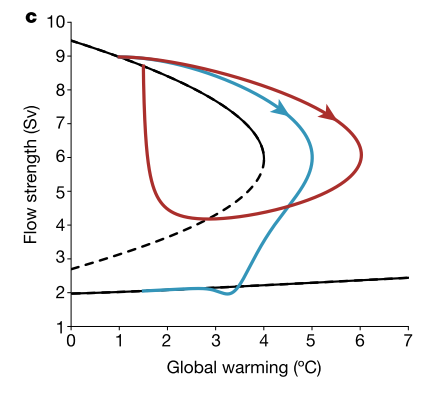
\includegraphics[width=0.7\linewidth]{Images/Metrics/overshoot_saving}
%	\caption{Example of a system avoiding full tipping, taken from \citep{Ritchie2021}. In this case the temperature grows very fast until $6$~C and then quickly goes back to $1.5$~C.As the temperature grows both the blue trajectory (slow forcing) and the red trajectory (fast forcing) go trough the bifurcation threshold. However the red trajectory manages to recover from the tipping thanks to the faster parameter change.}
%	\label{fig:overshootsaving}
%\end{figure}


\begin{figure}
	\centering
	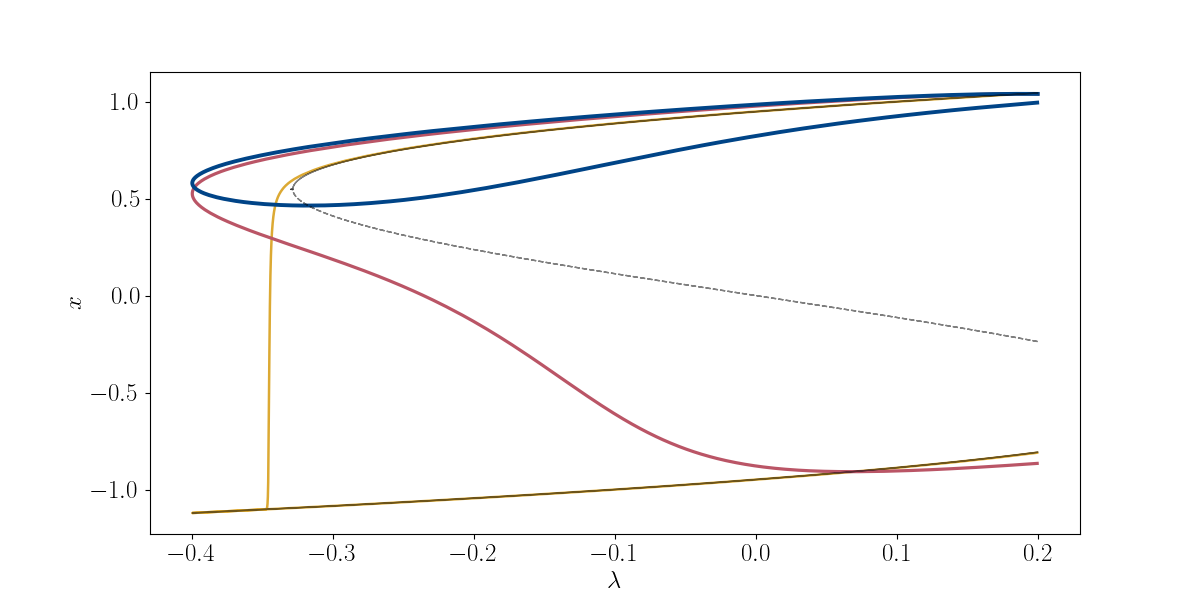
\includegraphics[width=0.9\linewidth]{Images/Metrics/overshoot2}
	\caption{Example of a system avoiding full tipping, inspired by \cite{Ritchie2021}, where a system's control parameter is swiped from an initial value, past a bifurcation value, and then is set back to the initial value.  In this case the yellow trajectory represents a slow sweeping of the control parameter, the red trajectory represents an intermediate sweeping speed where the system still tips, and the blue trajectory presents a fast sweep where the systems avoids tipping to the lower stable branch.   }
	\label{fig:overshootsaving}
\end{figure}



% 
%\begin{figure}[htp]
%	\centering
%	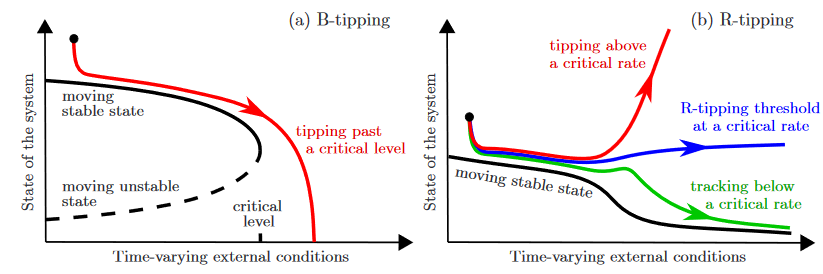
\includegraphics[width=0.9\linewidth]{Images/Metrics/exampl}
%	\caption{..}
%	\label{fig:exampl}
%\end{figure}

%
%\begin{figure}[htbp]
%	\begin{center}
%		\begin{tikzpicture}
%			\tzaxes(0,0)(5,4){State}{Potential}
%			\tzfn[black,line width=0.2mm,col1,opacity=0.4]{2*(\x-1)^2*(\x-3)^2+0.5*\x+0.03}[0.6:3.4]{ }[ar]
%			\tzfn[black, thick]{2*(\x-1)^2*(\x-3)^2+0.5*\x}[0.6:3.4]{ }[ar]
%		%	\tzfn[<-,black,dashed]{2*(\x-1)^2*(\x-3)^2+0.5*\x+0.3}[1.6:2.7]{ }[ar]
%		%	\tzfn[<-,very thick,col1,dashed]{2*(\x-0.2-1)^2*(\x-0.1-3)^2+0.5*(\x-0.2)-0.1}[3.1:3.4]{ }[ar]
%			%			\draw [->,thick](0.8,0) -- (0.3,0);
%			%			\draw [->,thick](-0.8,0) -- (-0.3,0);
%			%			\draw [->,thick](1.2,0) -- (1.5,0);
%			%			\draw [->,thick](-1.2,0) -- (-1.5,0);
%			\node (a) at (0,0) {};
%			\filldraw [col2,opacity=0.4] (0.97,0.5+0.14) circle [radius=0.1cm];
%			\filldraw [col2](2.97,1.5+0.14) circle [radius=0.1cm];
%			\filldraw [col2](3.2, 2.06 + 0.5) circle [radius=0.1cm];
%		%	\draw [<->,thick](0.4,1.5)--(0.4,2.9);
%		%	\draw [<->,thick](2.1,0.2)--(2.9,0.2);
%		%	\node (t) at (2.5,3.9) {High resiliance}[c];		
%		\end{tikzpicture} 
%		\begin{tikzpicture}
%			\tzaxes(0,0)(5,4){State}{Potential}
%
%			\tzfn[black,ultra thick,col1]{2*(\x-1)^2*(\x-3)^2+0.5*\x+0.01}[0.6:3.4]{ }[ar]
%			\tzfn[black, thick]{2*(\x-1)^2*(\x-3)^2+0.5*\x}[0.6:3.4]{ }[ar]
%			%			\draw [->,thick](0.8,0) -- (0.3,0);
%			%			\draw [->,thick](-0.8,0) -- (-0.3,0);
%			%			\draw [->,thick](1.2,0) -- (1.5,0);
%			%			\draw [->,thick](-1.2,0) -- (-1.5,0);
%			\node (a) at (0,0) {};
%			\filldraw [col2] (0.92,0.7+0.1) circle [radius=0.1cm];
%			\filldraw [col2,opacity=0.4](2.92,3*0.7+0.1) circle [radius=0.1cm];
%			\filldraw [col2] (3.22, 2.4 + 0.5) circle [radius=0.1cm];
%		%	\draw [<->,thick](0.4,2.1)--(0.4,2.5);
%		%	\draw [<->,thick](2.4,0.2)--(2.9,0.2);
%		%	\node (t) at (2.5,3.9) {Low resiliance}[c];		
%		\end{tikzpicture}
%	\end{center}
%	\caption{As the system(ball)  }
%	\label{fig: rate_intertial_picture}
%\end{figure}


%\input{Chapters/EWS_rate_tikz.tex}

%
%\begin{figure}[H]
%	\centering
%	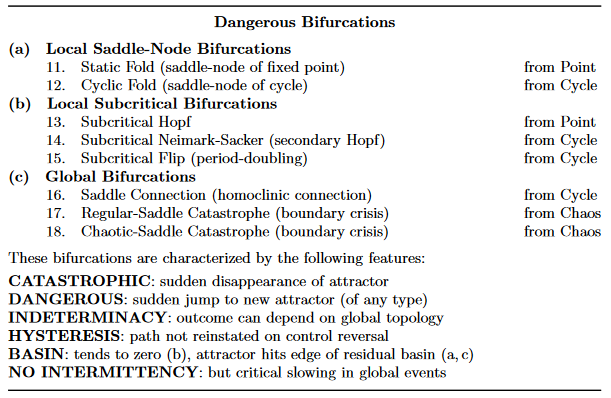
\includegraphics[width=0.9\columnwidth]{Images/Metrics/catastrofic_bifurc.png}
%	\caption{Dangerous bifurcations}
%	%	\caption{Events per ms}
%	\label{tab:dangerous_bifs}
%\end{figure}

Table \ref{tab:codim_1_prec} shows a list of possible precursors to  codimension-1 bifurcations. 

\begin{table}[H]
				\centering
	\begin{tabular}{lll}
		\hline
		\multicolumn{3}{c}{\textbf{Precursors of Codimension-1 Bifurcations }} \\
		Supercritical Hopf & S: point to cycle & LDR$\rightarrow 0$ linearly with control \\
		Supercritical Neimark & S: point to torus & LDR$\rightarrow 0$ linearly with control \\
		Supercritical flip & S: cycle to cycle & LDR$\rightarrow 0$ linearly with control \\
		Band merging & S: chaos to chaos & Separation decreases linearly \\
		Flow explosions & E: point to cycle & Path folds. LDR$\rightarrow 0$ linearly with control \\
		Map explosion & E: cycle to torus & Path folds. LDR$\rightarrow 0$ linearly with control \\
		Intermittency expl: flow & E: point to chaos & LDR$\rightarrow 0$ linearly with control \\
		Intermittency expl: map & E: cycle to chaos & LDR$\rightarrow 0$ as trigger \\
		Regular interior crisis & E: chaos to chaos & Lingering near impinging saddle cycle \\
		Chaotic interior crisis & E: chaos to chaos & Lingering near impinging saddle cycle \\
		Static fold & D: from point & Path folds. LDR$\rightarrow 0$ linearly with control  \\
		Cyclic fold & D: from cycle & Path folds. LDR$\rightarrow 0$ linearly with control \\
		Subcritical Hopf & D: from point & LDR$\rightarrow 0$ linearly with control \\
		Subcritical Neimark & D: from cycle & LDR$\rightarrow 0$ linearly with control \\
		Subcritical glip & D: from cycle & LDR$\rightarrow 0$ linearly with control \\
		Saddle connection & D: from cycle & Period of cycle tends to infinity \\
		Regular exterior crisis & D: from chaos & Lingering near impinging saddle cycle \\
		Chaotic exterior crisis & D: from chaos & Lingering near impinging accessible saddle \\
		\hline
	\end{tabular}
	\caption{Taken from \cite{Thompson2011a}.  }
	\label{tab:codim_1_prec}
\end{table}

%
%\begin{figure}[H]
%	\centering
%	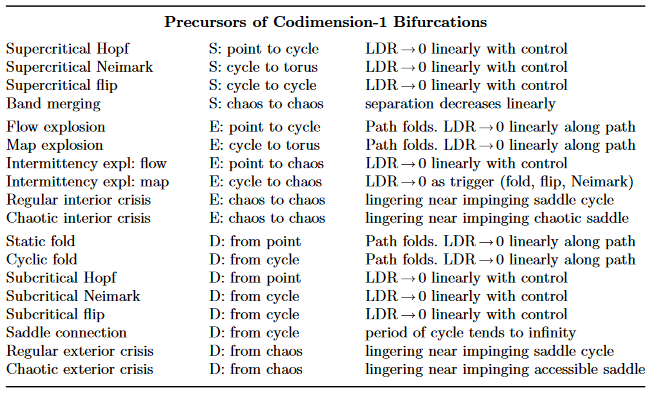
\includegraphics[width=0.9\columnwidth]{Images/Metrics/codim_1_precursors.png}
%	\caption{ safe bifurcations}
%	%	\caption{Events per ms}
%	\label{tab:codim_1_prec}
%\end{figure}

For now we will focus on codimension-1 parameters where the local Local Decay Rate (LDR) approaches 0, and situations where the system goes from a stable state to another. 




%\begin{figure}[hbtp]
%	\centering
%	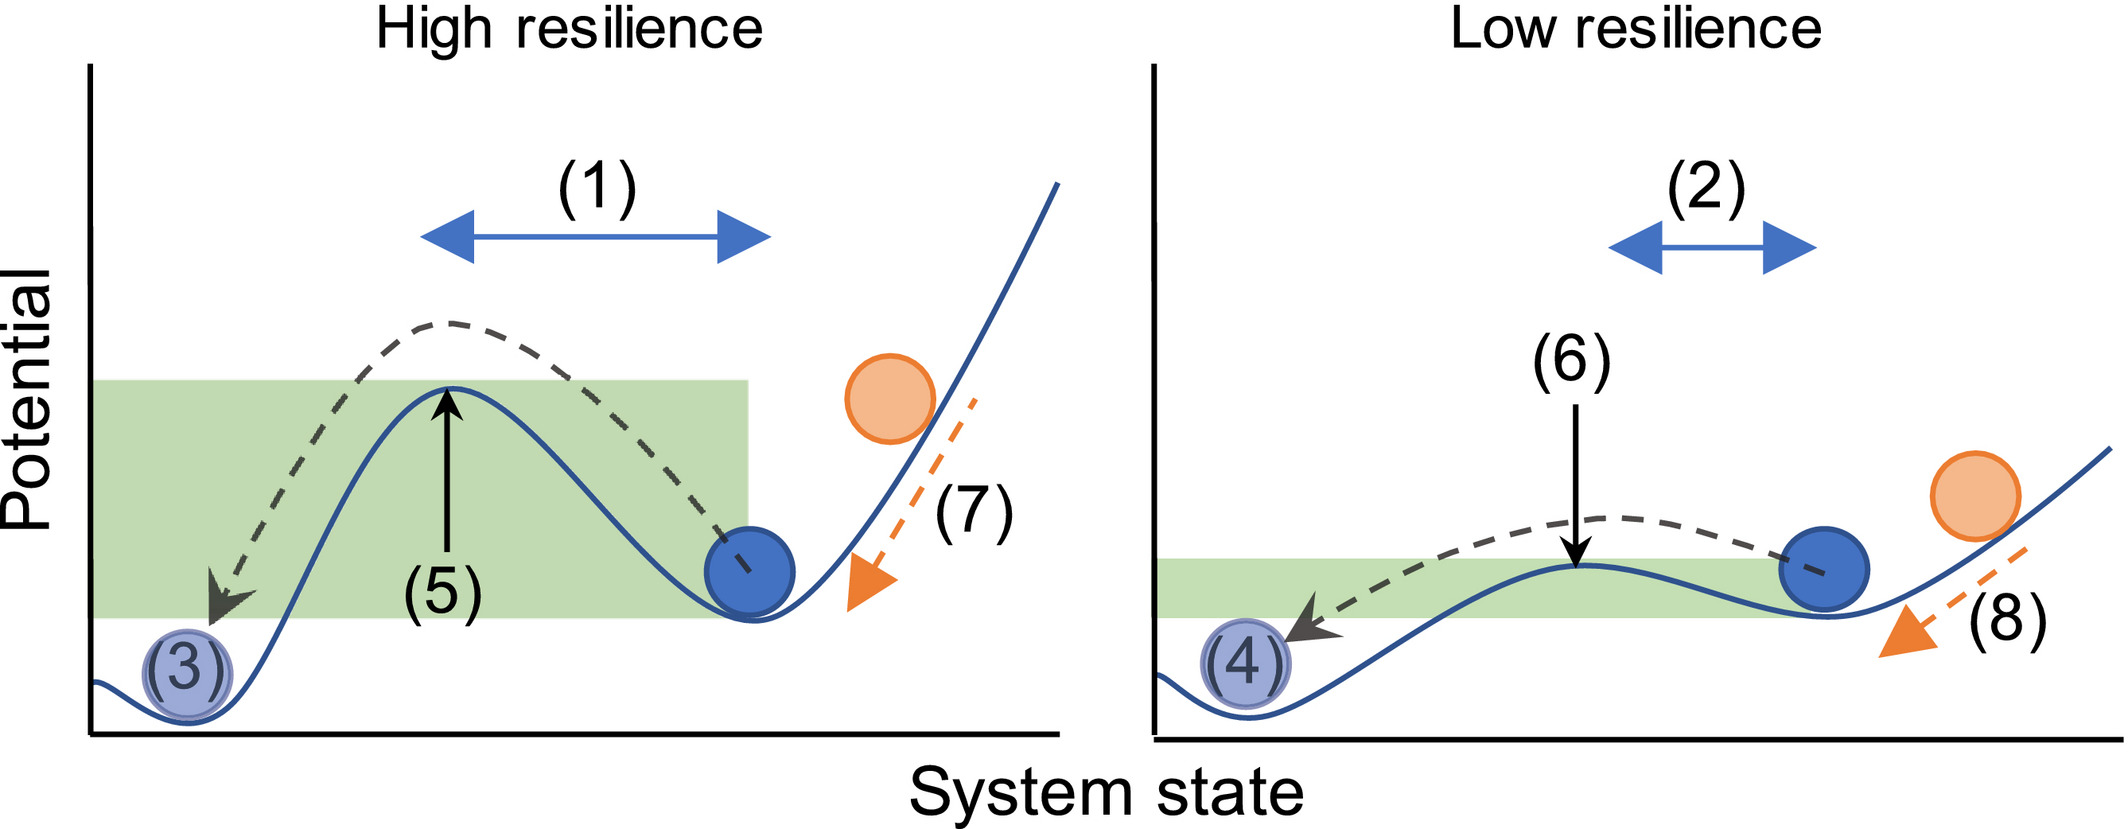
\includegraphics[width=.8\textwidth]{Images/Metrics/resiliance}
%	\caption{Resiliance figure from \cite{Clements2018a} }
%	\label{fig: resiliance}
%\end{figure}



%We can give an easy quantification of this for bifurcation where the eigenvalues are real and there is a change of sign\footnote{For complex valued bifurcations, like the Hopf bifurcation, a threshold timescale could be the slowest timescale of the cycle, or just the period}. 



%If the system is near en equilibrium and is perturbed by white noise with variance $\sigma$, then we can consider a perturbation of $2\sigma$, linearize about the stable state before the transition and estimate the relaxation time. 


%In this case $\dot{x}=f(x)=r(x-2)(x-1)(x-3)$, we linearize about $x=x^*=2$, and use an initial value $x_0=x^*\pm2\sigma=2\pm 2\sigma$.
%\begin{equation}
%	f|_{x^*}=f(x^*)+f'(x^*)(x-x^*) \rightarrow \dot{x}|_{x^*}=f(x^*)+f'(x^*)(x-x^*)
%\end{equation}
%then 
%
%\begin{equation}
%	x|_{x^*+2\sigma}=A e^{f'(x^*+2\sigma)t}+\frac{f(x^*+2\sigma)-f'(x^*+2\sigma)(x^*+2\sigma)}{f'(x^*+2\sigma)}
%\end{equation}
%
%so the characteristic timescale is $t^*=-\frac{1}{f'(x^*+2\sigma)}$.



%In this case the second term is related to the equilibrium, and it is exactly the equilibrium in the $\sigma\rightarrow 0$ limit. 
%This is irrelevant for our analysis, however is it worth noting that, if the analysis is valid, the equilibrium is decoupled (?) from the noise.


%
%Clearly this approximation breaks near the bifurcation since the system cannot be linearized, and the relaxation time goes diverges. However, according to this, the relaxation time is smaller with larger noise. 



%In general, in $n$ dimentions:

%\begin{equation}
%\begin{bmatrix}
%	x_1 \\
%	\vdots \\
%	x_n 
%\end{bmatrix}
%=
%\begin{bmatrix}
%	f_1(x_1, \hdots ,x_n) \\
%	\vdots \\
%	f_n(x_1, \hdots ,x_n)
%\end{bmatrix}
%\end{equation}

%Now we will have $n$ relaxation times given by the eigenvalues ($m_n$) of the Jacobian of the system.


%
%Then the relaxation time-scale is the slowest timescale, given by the dominant eigenvalue $m_{max}$.
%
%\begin{equation}
%	 t^*=-\frac{1}{m_{max}(\vec{x}^*)}
%\end{equation}

\subsection{Pure stochastic tipping, or N-tipping}

In this case there is no need for a changing parameter, we consider the system at a given value of the control $\la_0$, with stable equilibrium $x^*$  and respective basin of attraction ($\mathcal{B}(x^*)$). If this system has a noise with a standard deviation ($\mathrm{STD}(x)$), then there is a non zero probability for the system to escape the basin, or alternatively, an average escape time. 

%For additive noise, the system can be written as a Langevin equation 

If the local stable attractor has a local potential well with the smallest well height being $\Delta U$, then the  escape time is approximated by Kramers time: 
\begin{equation}
	t_k=c e^{2\Delta U/\mathrm{Var}^2}
\end{equation} 
Where Var denotes the variance of the system around $x^*$.

%There have been accounts \citep{bibid} where the importance of the noise to signal ratio is remarked for the performance of EWS. 
%This seems to point that this is not important and the relevant feature is the relation between the noise and the local landscape of the manifold, through the relaxation timescale. This is further evident when we consider we can translate the whole problem to whichever value we want\footnote{for example at $0$ ( $\dot{x}=f(x)=\la(x-1)(x)(x+1)$)}, then the signal to noise ratio for the stable point at the middle is infinite, but the normal form of the equation and all the dynamics remain the same. 

It should be noted that translations of the dynamical system work differently for additive or multiplicative noise.  
If a 1D system\footnote{Also true in higher dimension, but in 1D the states are ordered.} has two stable states for a given parameter ($x_+^*>x_-^*$) with additive noise of intensity $\sigma$ then all probabilities and dynamics are the same if translated\footnote{$dx=f(x,\la)\, dt+ \sigma dW$ and $dx=f(x+\mu,\la)\, dt+ \sigma dW$  have the same statistical properties.} to ($x_+^*+\mu>x_-^*+\mu$). 

However with multiplicative noise, translating the system not only changes the noise, but the probabilities of escaping from each well. A system with a state at $x_+=2$ has twice the noise of the state at  $x_-=1$, however it will have almost the same noise if translated to  $x_+=22$ and $x_-=21$.

Some works related to noise tipping can be found in \citep{Sharma2015}.

In this case the tipping cannot be predicted since it is the result of a purely random  process, however the probability of tipping can be studied.






\subsection{Rate induced bifurcations, or R-tipping}

Following the work done by \cite{Ashwin2012,Kees2017a,Kiers2020a}, if we consider a control parameter that changes with time $\la=\la(t)$ then the system of equations \eqref{eq: ODES} becomes a  non-autonomous system. 
Now the full dynamical system can be written as
\begin{equation}
	\begin{cases}
		d x&=f(x,\lambda) \, dt\\
		d \lambda&= c_\lambda(t,\la)\, dt
	\end{cases}
\label{eq:Aug1}
\end{equation}
which we call the augmented system of  equation \eqref{eq: ODES}.
 $c_\lambda(t,\la)$ is a $C^0$ function that does not depend on $x$. 
If $c_\lambda(t,\la) \neq 0$ this variable does not have a nullcline, therefore there  are no equilibria. However, we can study if the system can track the equilibrium of the autonomous system as the control parameter changes. 
In particular, we want to know for which parameter speeds the system can 'close track'  the autonomous equilibrium $x^*(\la)$. 

In this case, close tracking $x^*$ implies that the trajectories of the augmented system \cref{eq:Aug1}, also called pullback attractor $X(t)$,  are bounded around the expected equilibrium, that is $|X(t)-x^*(t)|<\epsilon$. 

In \cite{Ashwin2012} this deviation from $x^*$ is calculated assuming  a case where $M$ does not depend on the sweeped parameter
\begin{equation}
	X(t)=x^*(t)-\frac{1}{||M||}\frac{d x^*}{d\lambda}\frac{d\lambda}{d t }.
	\label{eq:r_equilibrium}
\end{equation}
where $\frac{1}{M}\frac{d x^*}{d\lambda}\frac{d\lambda}{d t }$ is  called the linear instantaneous lag ($L(t)$) and approximates the state of the pullback attractor $X$. 
They also develop a criterium for avoiding R-tipping in codimension-1 systems:
\begin{equation}
	\frac{1}{||M||} \left| \frac{d x^*}{d\lambda}\frac{d\lambda}{d t } \right| <R
\label{eq:Ashwin_track}
\end{equation}
where $\frac{d x^*}{d\lambda}\frac{d\lambda}{d t }=\frac{d x^*}{d t}$ and $R$ is an effective tipping radius, strictly smaller than the basin, that can depend not only on the basin volume but on the general shape of the potential, even far the stable point. 
For speeds $|\frac{d\lambda}{d t }|$ large enough, the system can R-tip to other behaviors by escaping the basin of attraction. 

In \cite{Kees2017a,Kiers2020a} a more relaxed notion of tracking is discussed, where the augmented systems only move the parameter from an initial value $\la_-$ on $x_-^*$ to a final value $\la_+$ on $x_+^*$. In this case if, after the change in the control parameter, the system relaxes to the same stable attractor ($x_+^*=x_-^*$ ), then we say it 'endpoint tracks' the initial attractor $x^*_-$, even if the system can  go through the autonomous basins of other attractors in  between. 
%In their work the notion of forward basin stability and forward inflowing stability are introduced to define constraints for endpoint tracking in special cases. 

In this sense, the red trajectory from \ref{fig:overshootsaving} could be said to endpoint track the original attractor, even if it does not close track. 

\cite{Pierini2021,Vanselow2019} also consider a temporary extreme excursion of the state far from the stable dynamics as an R-tipping effect.
It should be noted that this particular effect is only possible in more than 1 dimension since it is related to the shape of the potential,  being such that the path the system takes is not the shortest path to the equilibrium once the sweeping stops. 
In this case they refer to a loss of tracking to an evolution that has a transitory new behavior even if the end result is the same and no bifurcation separatrix is crossed.


\subsubsection{Intuitive interpretation}

A simple way to understand R-tipping is to think about the system as being in a surface similar to the potential of the system.
 
In the simple case where $M$ does not depend on the sweeping parameter we can think of a system as  

\begin{equation}
	\begin{cases}
		d x&=f(x-\lambda) \, dt\\
		d \lambda&= c_\lambda(t,\la)\, dt
	\end{cases}
	\label{eq:Aug2}
\end{equation}

Then the effect of  moving the parameter results in 'moving' the surface, so the equilibria (the local minima of the surface) moves as $\dot x^*$ and the system feels a non inertial force equal to  $\dot x^*/M$, as pictured in \cref{fig:slow}, where $c_\la=0$ at the initial and final time. 

\begin{figure}[bt]
	\centering
	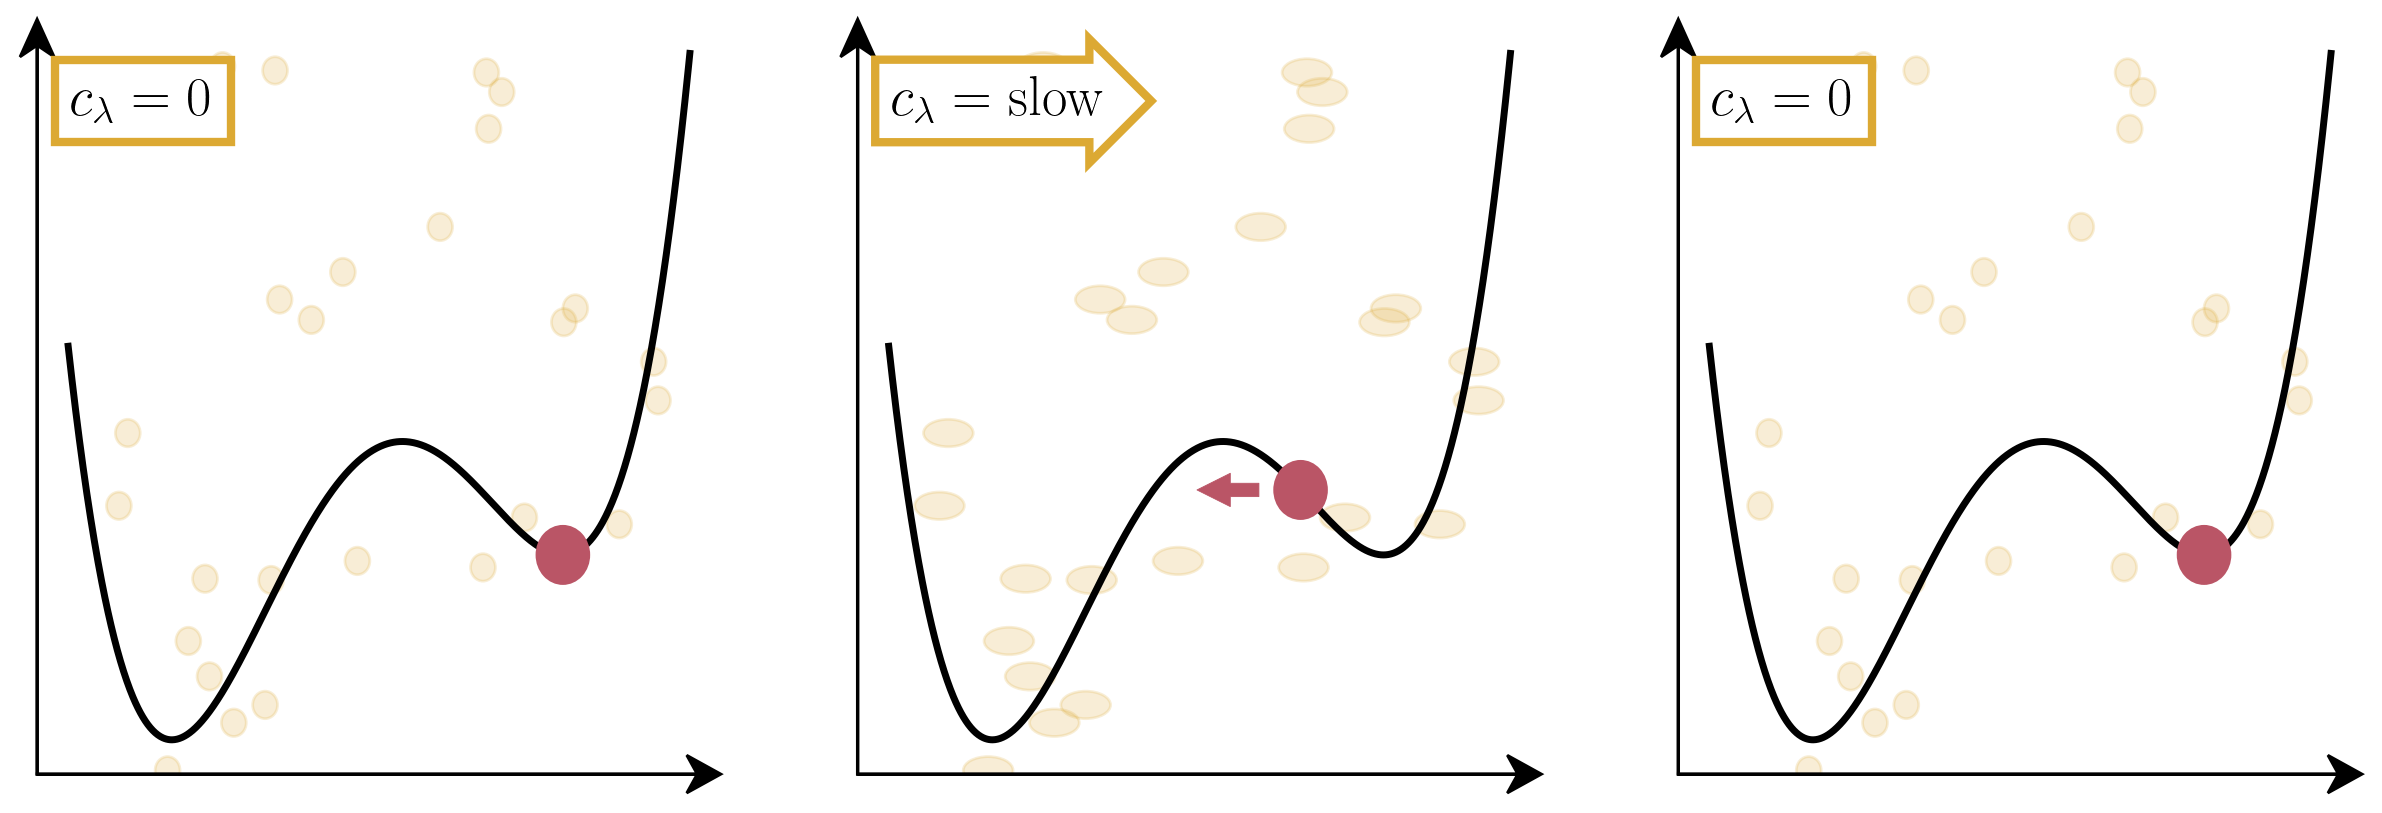
\includegraphics[width=\linewidth]{Images/Metrics/acceleration/slow}
	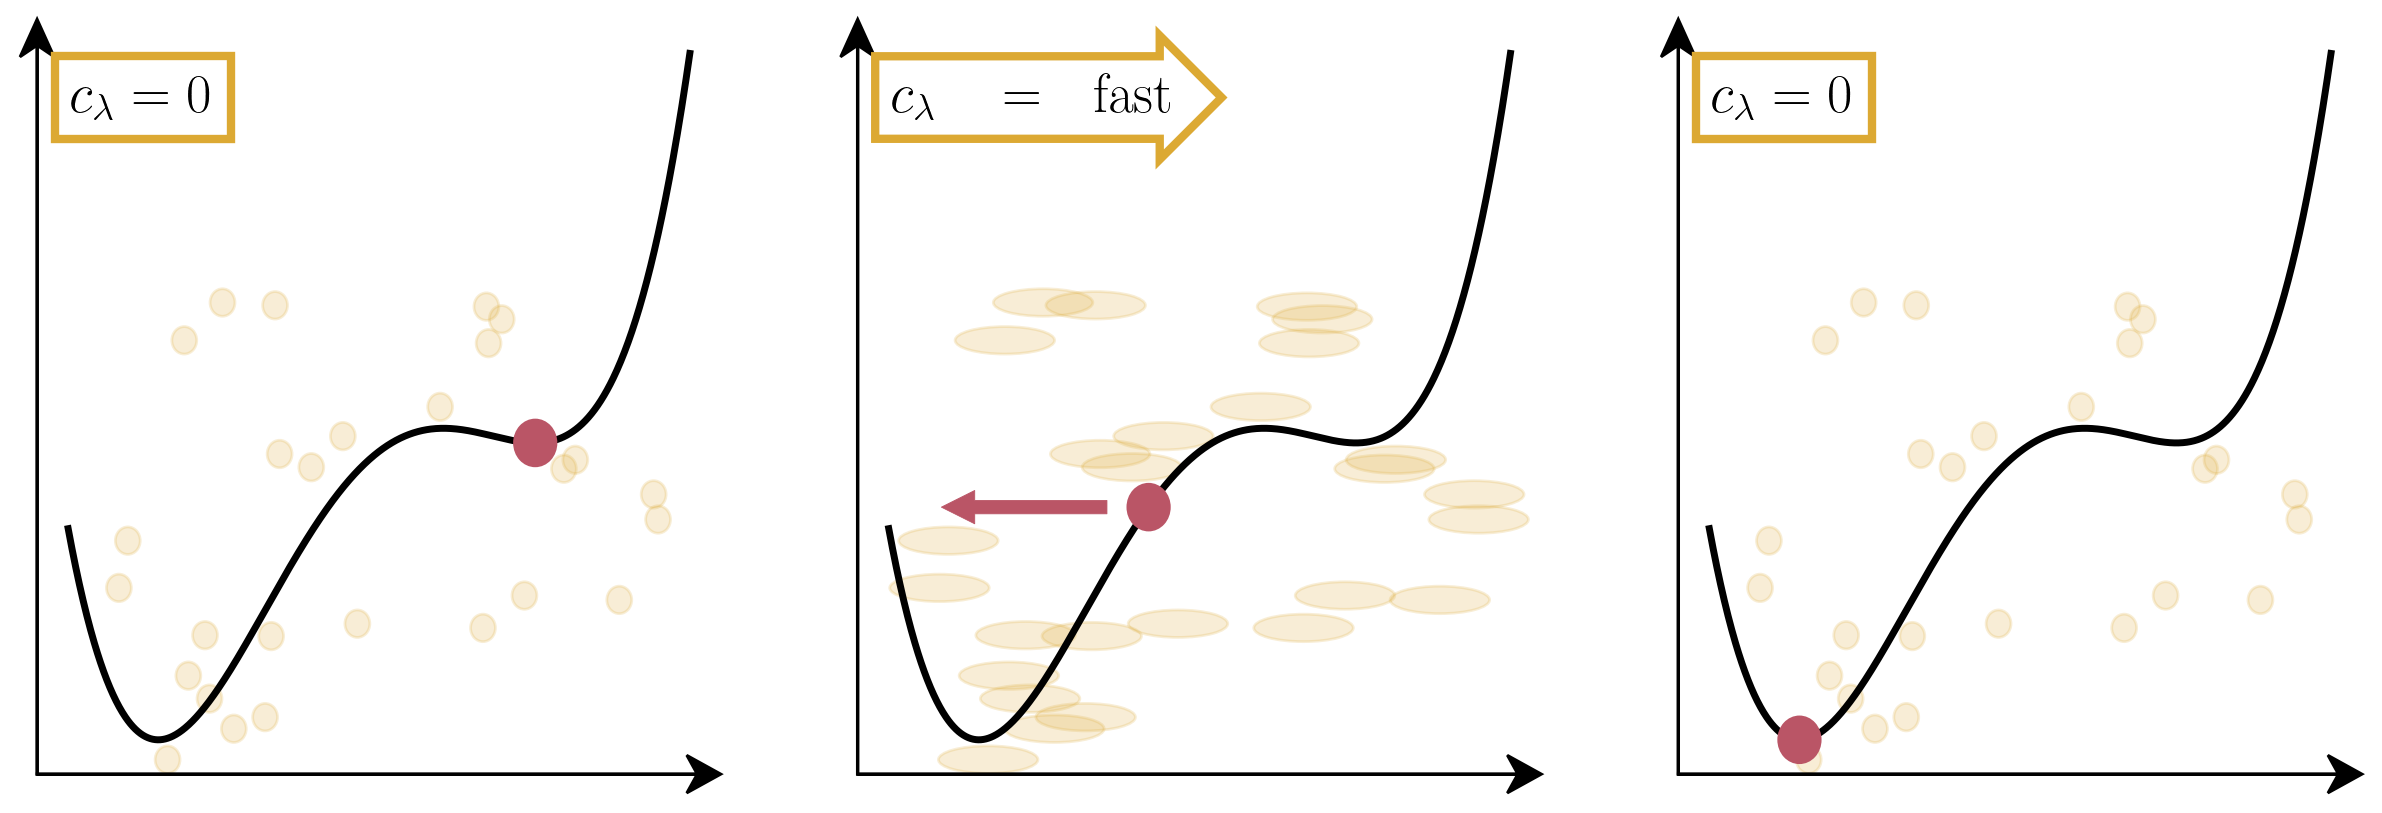
\includegraphics[width=\linewidth]{Images/Metrics/acceleration/fast}
	\caption{The effect of the sweeping parameter as the potential moves is like non-inertial force.  This scheme exemplifies a system that moves from one initial parameter to another, either slowly (top row) or fast (bottom row). In the fast case, the sweeping force tips the system (red) to the other equilibrium. The background yellow dots are there to show the movement of the surface.}
	\label{fig:slow}
\end{figure}

This idea gives an intuition on why \cref{eq:r_equilibrium} can still hold when $M(\la)$ as long as it stays close enough to the equilibrium.%, while for faster swipes the system will feel the slope of the rest of the surface. 


\subsection{Shock induced bifurcations, or S-tipping}

These are cases where an external shock, or an extreme event can kick the system out of its current basin of attraction \citep{Halekotte2020}.
\cite{Parry2022} discussed how, as the amazon forest loses resilience, a tipping might occur before   the global temperature (the control parameter), reaches the dynamical bifurcation and can be triggered by a  shock due to an extreme event, which in this case can be related to a large wildfire\footnote{This was proposed as a possible explanation by Peter Cox in a seminar \url{https://www.youtube.com/watch?v=kZqv3Tsew00&t=886s}}.  
The effect of shocks and extreme events as source of dynamical changes has been extensively studied as sources of tipping in financial markets   \citep{Sornette2009a}.

